%!TEX root=finmath1.tex
\chapter{Введение в NumPy}
\label{ch:numpy}
\chaptertoc

NumPy (Numerical Python) "--- это пакет для эффективной работы с массивами и матрицами, содержащий также функции линейной алгебры, генераторы случайных чисел и другие методы. 
NumPy позволяет существенно ускорить код на Python, что необходимо в приложениях в финансовой математике "--- без NumPy эффективная реализация финансовых моделей на Python практически невозможна.

Это занятие содержит введение в средства NumPy, которые нам потребуются в дальнейшем.
Не все они будут нужны сразу, поэтому рекомендуется ознакомится с занятием бегло, а потом возвращаться по мере необходимости.

\section{Основные принципы Numpy}
Чистый Python "--- медленный язык программирования и не подходит для приложений, где требуются интенсивные вычисления. 
Однако с помощью ряда пакетов (NumPy, SciPy и другие) этот недостаток можно преодолеть.
Основной принцип их использования состоит в том, что нужно переложить трудоемкие вычисления на функции, написанные на быстрых языках (в основном, C), которые могут легко вызываться из кода на Python.

Приведем пример.
Следующие две функции вычисляют вероятность того, что броуновское движение превысит уровень $x=1$ на отрезке $t\in[0,1]$ с помощью метода Монте-Карло.
Для этого они симулируют $m=10\,000$ траекторий, где каждая траектория представлена своими значениями в $n=100$ точках $\{0.01, 0.02, \dots, 1\}$, а затем вычисляют долю траекторий, превысивших уровень (сейчас можно не обращать внимания на детали реализации, нам будут важны лишь общие принципы).

\begin{python}
### numpy-basics.ipynb ###
from random import gauss
# ... [другие импорты]

def slow_function(x, m, n):
    sigma = 1/sqrt(n)
    count = 0
    for i in range(m):  # итерация по траекториям
        W = 0
        for j in range(n):  # итерация по времени
            W = W + gauss(0, sigma)
            if W >= x:
                count += 1
                break
    return count/m

def fast_function(x, m, n):
    rng = np.random.default_rng()             # генератор случайных чисел
    dW = rng.normal(0, 1/sqrt(n), size=(m,n)) # приращения броуновского движения
    W = np.cumsum(dW, axis=0)                 # траектории броуновского движения
    return np.mean(np.any(W >= x, axis=0))    # доля траекторий, превысивших 1
\end{python}

Медленная функция представляет собой стандартный способ генерации траекторий во вложенном цикле, где шаг внутреннего цикла соответствует очередному приращению траектории, а внешний цикл производит нужное количество траекторий.
Для $m=10\,000$ и $n=100$ блок кода во внутреннем цикле выполняется порядка миллион раз\footnote{На самом деле меньше, так как внутренний цикл будет прерван при превышении $x$.}.

Быстрая функция устроена по-другому.
Она состоит из трех крупных операций: сначала генерируются приращения сразу всех траекторий, затем из массива приращений строятся траектории броуновского движения, и наконец считается доля нужных нам траекторий.
Эти операции выполняются функциями NumPy, которые вызывают внутри себя быстрый код на С.
И хотя объем вычислительной работы остался таким же (по-прежнему нужен миллион реализаций нормальной случайной величины), это делается быстрее, чем на чистом Python.

Для измерения скорости работы этих двух функций в ноутбуке в Jupyter можно воспользоваться командами \verb"\%timeit slow_function(1, 10000, 100)" и \verb"\%timeit fast_function(1, 10000, 100)".
Получится различие примерно в 10--20 раз.

Техника вычислений, примененная в быстрой функции, называется \emph{векторизацией}.
Она предполагает работу не с каждым значением по отдельности, а сразу с массивом значений.
С помощью грамотного применения векторизации можно достичь скорости работы, сравнимой со скоростью быстрых языков типа C, при этом сохранив простоту и удобство Python.

При использовании векторизации центральное место занимают различные операции с массивами.
Их мы и будем рассматривать в этом занятии.


\section{Основные операции с массивами в NumPy}

\subsection{Создание массивов}
Массив NumPy можно создать из списка с помощью применения функции \verb"array".
Вложенные списки дают многомерные массивы.
Вместо списков можно использовать кортежи.
\begin{python}
# Пример одномерного и двумерного массива
a = np.array([1, 2, 5, 10])
b = np.array([[1, 0], [0, 1], [1, 1]])
\end{python}

У каждого массива есть аттрибуты \verb"size" (количество элементов), \verb"ndim" (количество измерений "--- они называются \emph{осями} массива), \verb"shape" (форма).
Форма является кортежем натуральных чисел, которые обозначают длину массива вдоль каждой оси.
Например, форма одномерного массива "--- это одно число (кортеж длины 1), двумерного массива "--- пара чисел, и \td
\begin{python}
print(a.ndim, a.shape, a.size)  # 1 (4,) 4 
print(b.ndim, b.shape, b.size)  # 2 (3, 2) 6
\end{python}
Следующие функции создают массивы специального вида:
\begin{itemize}
\item \verb"np.zeros(shape)" "--- массив из нулей заданной формы;
\item \verb"np.ones(shape)" "--- массив из единиц;
\item \verb"np.empty(shape)" "--- неинициализированный массив%
\footnote{Будет содержать бессмысленные значения, которые имелись в области памяти.
Функция \verb"empty" работает немного быстрее, чем \verb"np.zeros" или \verb"np.ones", поэтому ее можно использовать, когда требуется заранее выделить память под массив, который потом будет заполнен вручную.};
\item \verb"np.arange(start, stop, step=1)" "--- работает как стандартная функция Pyt\-hon \verb"range", но возвращает  массив NumPy, при этом вызов \verb"np.arange(n)" равносилен \verb"np.arange(0, n, 1)", \te\ возвращает массив чисел от 0 до $n-1$ включительно;
\item \verb"np.linspace(start, stop, num)" "--- равномерное разбиение отрезка на заданное количество точек.
\end{itemize}

\begin{python}
c = np.zeros(5)            # [0, 0, 0, 0, 0]
d = np.ones((3, 2))        # [[1, 1], [1, 1], [1, 1]]
e = np.arange(5)           # [0, 1, 2, 3, 4]
f = np.arange(0, 10, 2)    # [0, 2, 4, 6, 8]
g = np.linspace(0, 1, 11)  # [0, 0.1, 0.2, 0.3, 0.4, 0.5, 0.6, 0.7, 0.8, 0.9, 1]
\end{python}

\begin{remark}
Здесь и далее, когда нужно показать в комментариях, что результатом операции является двумерный массив, будет использоваться запись вида \verb"[[x11, x12, ...], [x21, x22, ...], ...]", в которой внутренние списки соответствуют строкам массива.
\end{remark}

\begin{remark}
Функция \verb"linspace" полезна для вычисления некоторой математической функции на заданном отрезке, когда нужны сразу все ее значения "--- например, чтобы построить график.
Часто встречается код следующего вида.
\begin{python}
X = np.linspace(a, b, n)
plt.plot(X, f(X))   # график функции f на отрезке [a, b]
\end{python}
Здесь функция \verb"f" должна быть \emph{универсальной}, \te\ возвращать массив при применении к массиву (об универсальных функция сказано далее).
Функция \verb"plot" "--- это стандартный способ построения графиков из пакета \verb"matplotlib".
Первый ее аргумент принимает массив $x$-координат, второй "--- массив $y$-координат.
\end{remark}

Иногда бывает нужно менять форму массива, сохраняя его элементы.
Это можно сделать методом \verb"reshape".
Метод \verb"flatten" разворачивает многомерный массив в одномерный, содержащий все элементы исходного массива, проходя слева направо и сверху вниз.
\begin{python}
np.arange(6).reshape((3, 2))          # [[1, 2], [3, 4], [5, 6]]
np.array([[1, 5], [2, 6]]).flatten()  # [1, 5, 2, 6]
\end{python}

Если при вызове \verb"reshape" по какой-то оси указать длину $-1$, то соответствующая длина будет рассчитана автоматически, исходя из размера всего массива.
Например, в примере выше можно написать \verb"np.arange(6).reshape((3, -1))" или \verb"np.arange(6).reshape((-1, 2))".


\subsection{Доступ к элементам массива. Срезы. Транспонирование}
Элементы массива можно получить с помощью квадратных скобок: \verb"x[i]" "--- это 
элемент массива \verb"x" с индексом $i$.
Индексация начинается с нуля.
Разрешены отрицательные индексы: $\verb"x[-1]"$ "--- это последний элемент массива, \verb"x[-2]" "--- предпоследний, и \td.

Для двумерных массивов $\verb"x[i, j]"$ означает элемент в $i$-й строке и $j$-м столбце.
Для трёхмерных массивов \verb"x[i, j, k]" "--- это элемент в $i$-й строке, $j$-м столбце и $k$-й <<глубине>>.
Для массивов большей размерности аналогично.

Чтобы получить всю строку или весь столбец двумерного массива, можно использовать запись \verb"x[i, :]" или \verb"x[:, j]".
Двоеточие здесь означает, что нужно взять все элементы вдоль соответствующей оси.
Аналогично для массивов с большим числом измерений. 
Если в индексации $n$-мерного массива указать $k<n$ индексов, то они будут отсчитаны по первым $k$ осям, а по оставшимся осям будут взяты все индексы.
Например, если массив \verb"x" двумерный, то \verb"x[0]" "--- это нулевая строка (то же самое, что \verb"x[0, :]"; а если трехмерный, то это уже двумерный массив \verb"x[0, :, :]").

\emph{Срезом массива} (slice), называется его подмассив определенного размера.
Срез одномерного массива задается в виде \verb"x[i:j]", где $i$ "--- индекс первого элемента среза, а $j$ "--- индекс первого элемента после среза (элемент с индексом $j$ не включается).
Например, \verb"x[1:4]" "--- это срез, содержащий элементы с индексами 1, 2 и 3.
Если индекс $i$ опущен, срез начинается с начала массива.
Если индекс $j$ опущен, срез заканчивается в конце массива.

Чтобы получить каждый $n$-й элемент, используется синтаксис \verb"x[i:j:n]".
Например, \verb"x[1:10:2]" "--- это срез, содержащий элементы с индексами 1, 3, 5, 7 и 9, а \verb"x[::3]" "--- каждый третий элемент.

Для двумерного массива можно использовать синтаксис \verb"x[i:j, k:l]" для получения среза, содержащего строки с индексами от $i$ до $j-1$ и столбцы с индексами от $k$ до $l-1$ включительно.
Можно также указать шаг, с которым будут выбираться строки или столбцы.
Для массивов с тремя и большим числом измерений все аналогично.

Для многомерных массивов иногда удобна индексация с использованием многоточия, позволяющая пропускать промежуточные оси, по которым будут взяты все значения индексов.
Например, \verb"x[..., 0]" эквивалентно \verb"x[:, :, 0]" для трехмерного массива, а \verb"x[1, 2, ..., 0]" эквивалентно \verb"x[1, 2, :, :, 0]" для пятимерного массива. 

Срезы являются полноценными массивами%
\footnote{Но при создании среза не происходит копирование значений в новую область памяти, поэтому взятие среза "--- быстрая операция.
Если же нужно именно создать новый массив, то можно воспользоваться методом \verb"copy": например, \verb"x[1:5].copy()".},
поэтому с ними можно проделывать все операции, которые мы рассмотрим дальше%
.
При этом оператор присваивания \verb"=", примененный срезу, изменит значения и в исходном массиве. 
Например, \verb"x[1:4] = 0" присваивает значение 0 элементам массива \verb"x" с индексами 1, 2 и 3.
Срезу можно присвоить и массив: например, \verb"x[1:4] = y" (формы среза и массива должны совпадать).

Транспонирование массива можно осуществить функцией \verb"np.transpose": если \verb"x" "--- двумерный массив (матрица), то \verb"np.transpose(x)" вернет транспонированную матрицу.
Если \verb"x" "--- одномерный массив, то вернется он сам; о поведение этой функции для массивов с тремя или более измерениями см.~документацию\footnote{\url{https://numpy.org/doc/stable/reference/generated/numpy.transpose.html}}.

Для транспонирования можно также использовать аттрибут \verb"T" массива, \te\ \verb"x.T".
Отличие от функции \verb"transpose" состоит в том, что \verb"T" возвращает представление того же массива и, например, присваивание его элементам новых значений изменит исходный массив.
Функция \verb"transpose" возвращает копию массива.

\begin{python}
# Индексация одномерного массива
x = np.arange(10)                     # [0, 1, 2, ..., 9]
print(x[5])                           # 5
print(x[-1])                          # 9
print(x[1:7:2])                       # [1, 3, 5]
x[1] = 100                            # Присваивание изменяет элемент массива
print(x)                              # [0, 100, 2, 3, ..., 9]

# Индексация двумерного массива
y = np.arange(10).reshape((2, 5))     # [[0, 1, 2, 3, 4], [5, 6, 7, 8, 9]]
print(y[0])                           # [0, 1, 2, 3, 4]
print(y[:,::3])                       # [[0, 3], [5, 8]] 

# Транспонирование
print(y.T)                            # [[0, 5], [1, 6], [2, 7], [3, 8], [4, 9]]
\end{python}


\subsection{Конкатенация массивов}
Функция \verb"np.concatenate((a1, a2, ...), axis)" конкатенирует (соединяет) массивы \verb"a1", \verb"a2" и \td\ вдоль измерения \verb"axis" (по умолчанию, \verb"axis=0"), при этом массивы должны иметь одинаковы формы, за исключением длины по измерению \verb"axis".
Например, если \verb"ai" "--- одномерные массивы, то они просто соединяются в новый одномерный массив.
Если массивы \verb"ai" двумерные, то при \verb"axis=0" они соединяться сверху вниз, а при \verb"axis=1" слева направо (в первом случае все массивы должны иметь одинаковое число столбцов, а во втором "--- одинаковое число строк).

Часто бывает нужно поставить одномерные массивы <<один на другой>>.
Для этого можно воспользоваться функцией \verb"np.vstack((a1, ..., an))", где \verb"ai" "--- одномерные массивы%
\footnote{Эквивалентно, можно сначала преобразовать массивы в двумерные, а затем применить \verb"concatenate", \te\ \verb"np.concatenate((a1.reshape((1, -1)), ... , an.reshape((1, -1))))".}.

\begin{python}
# Конкатенация одномерных массивов
x = np.array([1, 2])
y = np.array([3, 4])
print(np.concatenate((x, y)))  # [1, 2, 3, 4]
print(np.vstack((x, y)))       # [[1, 2], [3, 4]]

# Конкатенация двумерных массивов
x = np.array([[1, 2]])
y = np.array([[3, 4], [5, 6]])
print(np.concatenate((x, y)))            # [[1, 2], [3, 4], [5, 6]]
print(np.concatenate((x, y), axis=1))    # ошибка: у массивов разное число строк
print(np.concatenate((x.T, y), axis=1))  # [[1, 3, 4], [2, 5, 6]]
\end{python}


\subsection{Арифметические операции}
Арифметические операции  с массивами выполняются \emph{поэлементно}.
Например, \verb"x + y" "--- это массив, $i$-й элемент которого является суммой $i$-х элементов массивов \verb"x" и \verb"y". Массивы \verb"x" и \verb"y" могут иметь разную форму, но тогда будет осуществлен \emph{бродкастинг} (см.~далее).
То же самое верно для вычитания, умножения, деления и возведения в степень\footnote{Операция возведения в степень: \verb"x**y".}.
Для вычисления поэлементного максимума и минимума используются функции \verb"np.maximum(x, y)", \verb"np.minimum(x, y)".
Если один из аргументов \verb"x" или \verb"y" "--- скалярная величина, то операция с ней применяется к каждому элементу массива.

Чтобы получить матрицу $A_{ij} = x_i+y_j$ нужно применить \emph{внешнюю} операцию сложения $\verb"np.add.outer(x, y)"$ к одномерным массивам $\verb"x"$, $\verb"y"$.
Аналогичным образом работают \verb"np.multiply.outer", \verb"np.subtract.outer", \verb"np.divide.outer", \verb"np.power.outer", \verb"np.maximum.outer", \verb"mp.minimum.outer".
Их можно применять и к многомерным массивам, подробности см.~в документации\footnote{\url{https://numpy.org/doc/stable/reference/generated/numpy.ufunc.outer.html}}. 

Для скалярного произведения одномерных массивов используется функция \verb"np.dot(x, y)", для матричного умножения двумерных массивов используется она же, либо, эквивалентно, функция \verb"np.matmul(x, y)", либо оператор $\verb"x @ y"$.
Они могут применяться и к массивам с более чем двумя измерениями, при этом их поведение будет отличаться (подробнее см.~документацию\footnote{\url{https://numpy.org/doc/stable/reference/generated/numpy.matmul.html}}).

Отметим, что по умолчанию перечисленные операции создают новые массивы в памяти.
Таким образом, чтобы, скажем, увеличить значение всех элементов массива на 1, нужно выполнить еще операцию присваивания: $\verb"x = x+1"$.
Если массив большой, то эффективнее воспользоваться операцией инкремента и присвоения \verb"x += 1" (аналогично работают \verb"*=", \verb"-=", \verb"/=", \verb"**="), так как не будет создаваться промежуточный массив \verb"x+1".
\begin{python}
x = np.arange(4)                                     # [0, 1, 2, 3]
y = np.ones(4)                                       # [1, 1, 1, 1]
print(x+y)                                           # [1, 2, 3, 4]
print(np.maximum(x, y))                              # [1, 1, 2, 3]
print(np.add.outer([0, 1], [1, 2]))                  # [[1, 2], [2, 3]]
print(np.dot(x, y))                                  # 6
print(np.dot(x.reshape((2, 2)), y.reshape((2, 2))))  # [[1, 1], [5, 5]]
\end{python}


\subsection{Функции, применяемые к одному массиву}
Перечислим некоторые полезные стандартные функции, применяемые к одному массиву\footnote{В качестве аргументов эти функции могут принимать и обычные списки или кортежи, при этом их поведение будет таким же, как при передаче массивов такой же формы.}.
\begin{itemize}
\item \verb"np.sum", \verb"np.prod" "--- сумма и произведение всех элементов массива.
\item \verb"np.mean", \verb"np.std", \verb"np.var" "--- среднее, стандартное отклонение и дисперсия%
\footnote{Для дисперсии по умолчанию  используется формула $\frac1n \sum_{i=1}^n (x_i-\bar x)^2$, где $\bar x$ "--- среднее. Вызов \verb"np.var(x, ddof=1)" дает формулу, где в знаменателе стоит $n-1$ (\te\ несмещенную оценку дисперсии): \verb"ddof" означает degrees of freedom (количество степеней свободы).
То же самое верно для \verb"np.std".}.
\item \verb"np.min", \verb"np.max" "--- наименьший и наибольший элементы.
\item \verb"np.argmin", \verb"np.argmax" "--- индекс наибольшего и наименьшего элемента.
\item \verb"np.cumsum", \verb"np.cumprod" "--- кумулятивная сумма и произведение, \te\ если $x$ "--- одномерный массив, то \verb"np.cumsum(x)" будет иметь ту же длину и состоять из элементов \verb"x[0]", \verb"x[0]+x[1]", \verb"x[0]+x[1]+x[2]", и \td\ 
Если массив $x$ многомерный, то результат все равно будет одномерным и будет иметь длину, равную размеру $x$ (если не указан параметр \verb"axis", см.~ниже).
\item \verb"np.diff" "--- последовательная разность соседних элементов, \te\ массив из элементов \verb"x[1]-x[0]", \verb"x[2]-x[1]", \ldots, имеющий длину на 1 меньше, чем исходный массив.
\end{itemize}

Эти функции принимают дополнительный аргумент \verb"axis".
Если \verb"axis=None" (значение по умолчанию), функция применяется ко всем элементам массива.
Если \verb"axis" "--- число, то функция применяется вдоль этой оси.
Нумерация осей начинается с нуля.
Например, если \verb"x" "--- двумерный массив, то \verb"np.sum(x, axis=0)" вычисляет сумму элементов каждого столбца.
Результатом будет одномерный массив такой длины, сколько столбцов было в исходном массиве.
Аналогично, \verb"np.sum(x, axis=1)" вычисляет сумму всех элементов каждой строки массива \verb"x". 
\begin{python}
x = np.arange(4)
y = np.array([[1, 1], [2, 3]])
print(np.sum(x), np.sum(y))                # 10, 7
print(np.min(x), np.min(y))                # 1, 1
print(np.cumsum(x), np.cumsum(y))          # [0, 1, 3, 6], [1, 2, 4, 7]
print(np.sum(y, axis=0))                   # [3, 4]
print(np.cumsum(y, axis=0))                # [[1, 3], [1, 4]]
\end{python}


\subsection{Сохранение и загрузка из файла}
Для записи массива в файл или чтения массива из файла используются функции \verb"np.savetxt(filename)" и \verb"np.loadtxt(filename)".
Обе они записывают/читают один массив из одного файла.
Если требуется записать несколько массивов в один файл, нужно их сначала объединить в один. 

Эти функции принимают также дополнительный аргумент \verb"delimiter", которым будут разделяться значения. 
По умолчанию он равен символу пробела, но его можно изменить, например, на запятую, что удобно при просмотре файлов в Excel в виде csv-файлов.
Имеется также параметр \verb"fmt", который задает формат записи чисел.

У функции \verb"loadtxt" имеются дополнительные параметры \verb"usecols" и \verb"unpack", которые удобны при загрузке двумерных массивов.
Первый принимает список столбцов, которые нужно загрузить (остальные столбцы будут проигнорированы). 
Второй принимает значение \verb"True" или \verb"False"; если \verb"unpack=True", то функция вернет список массивов, где каждый элемент списка соответствует столбцу в файле (это удобно, если нужно присвоить им разные имена переменных), а если \verb"unpack=False" (по умолчанию), то вернется двумерный массив.
\begin{python}
# Значения синуса и косинуса на отрезке [0, 1]
x = np.linspace(0, 1, 101)
y = np.sin(x)
z = np.cos(x)

np.savetxt('sincos.txt', np.vstack([x, y, z]).T, fmt='%.3f', delimiter=',')
# Файл будет содержать столбцы x, sin(x), cos(x):
# 0.000,0.000,1.000
# 0.100,0.100,0.995
# 0.200,0.199,0.980
# ...

# Загрузим только значения x и косинуса, а затем построим график
t, f = np.loadtxt('sincos.txt', delimiter=',', usecols=(0, 2), unpack=True)
plt.plot(t, f)
\end{python}


\subsection{Случайные числа}
Для получения массива случайных чисел нужно сначала создать объект генератора случайных чисел, а затем вызвать его метод, производящий случайную выборку из соответствующего вероятностного распределения. 
В большинстве случаев подойдет стандартный генератор \verb"np.random.default_rng()".

Перечислим некоторые часто используемые распределения.
Далее \verb"rng" обозначает созданный генератор случайных чисел.
Все приводимые ниже методы принимают дополнительный аргумент \verb"size", задающий форму выходного массива, который будет заполнен независимыми реализациями случайной величины с соответствующим распределением.
По умолчанию \verb"size=None", что возвращает скаляр.
\begin{itemize}
\item \verb"rng.normal(loc, scale)" "--- нормальное распределение со средним значением \verb"loc" и стандартным отклонением \verb"scale";
\item \verb"rng.standard_normal()" "--- стандартное нормальное распределение;
\item \verb"rng.uniform(low, high)" "--- непрерывное равномерное распределение на отрезке [\verb"low", \verb"high"];
\item \verb"rng.binomial(n, p)" "--- биномиальное распределение в схеме из \verb"n" повторений с вероятностью успеха \verb"p";
\item \verb"rng.exponential(scale)" "--- экспоненциальное распределение с параметром $\lambda=$\,\verb"scale".
\end{itemize}

\begin{python}
rng = np.random.default_rng()
# массив 2x2 с нормально распределенными элементами
x = rng.standard_normal(size=(2,2))
# далее можно продолжать использовать уже созданный генератор
y = rng.uniform(0, 1, size=10)
# и т.д.
\end{python}

\begin{remark}
\label{np:r:seed}
Функции \verb"default_rng" можно передать параметр \verb"seed", который инициализирует алгоритм генерации  случайной последовательности%
\footnote{На самом деле, числа не случайные, а \emph{псевдослучайные} "--- они получаются по определенному алгоритму, у которого \verb"seed" задает начальное состояние.}.
Это полезно, когда нужен воспроизводимый результат: если создать генератор с заданным значением \verb"seed", то каждый раз он будет выдавать одну и ту же последовательность случайных чисел.
Если \verb"seed" не указывать, то он выбирается случайным образом из пула энтропии операционной системы, и при очередном исполнении кода генерируемые случайные числа будут различаться.
\end{remark}

\begin{remark}
Еще больше вероятностных распределений можно найти в пакету \verb"scipy.stats".
\end{remark}


\section{Векторизованные вычисления}
\subsection{Бродкастинг}
\emph{Бродкастинг} "--- это механизм, который позволяет NumPy работать с массивами разных форм при выполнении различных операций.
Например, если прибавить скаляр к массиву, то скаляр добавится к каждому элементу массива.
Если прибавить одномерный массив длины $n$ к двумерному массиву формы $(m,n)$, то первый массив добавляется к каждой строке второго.

Чтобы применить бродкастинг, формы массивов должны быть согласованными "--- удовлетворять определенному правилу.
Мы не будем здесь описывать механизм бродкастинга во всех деталях, а приведем лишь частный случай, который дальше будет часто встречаться (детали см.~в документации\footnote{\url{https://numpy.org/doc/stable/user/basics.broadcasting.html}}).

Если массив \verb"x" имеет форму \verb"(an, ..., a2, a1)", а массив \verb"y" имеет форму \verb"(bk, ...,  b2, b1)" и $k \le n$, то к ним можно применить бродкастинг, если \verb"a1"$=$\verb"b1", \verb"a2"$=$\verb"b2", \ldots, \verb"ak"$=$\verb"bk". 
Применяемая операция, скажем сложение, тогда будет прибавлять весь массив \verb"y" к каждому срезу массива \verb"x" вида \verb"x[an, ..., ad]", где $d=n-k$. Результатом будет массив с такой же формой, как у \verb"x". 
Если же $n < k$, то, аналогично, весь массив \verb"x" будет складываться с соответствующим срезом массива \verb"y" и форма результата будет такая же, как у \verb"y".

\begin{python}
# Массив x прибавляется к каждой строке y
x = np.arange(5)
y = np.arange(10).reshape((2, 5))
print(x+y)  # [[0,  2,  4,  6,  8], [10, 12, 14, 16, 18]]

# Следующий фрагмент приведет к ошибке, так как формы не согласованы
z = y.reshape((5, 2))
print(z + y)
\end{python}


\subsection{Универсальные функции}
\emph{Универсальной функцией} называется функция, которая применяется к каждому значению массива и возвращает массив (той же формы), заполненный результатами ее вычисления.
Универсальные функции дополнительно реализуют удобные методы, наподобие \verb"outer" (см.~выше); подробности см.~в документации\footnote{\url{https://numpy.org/doc/stable/user/basics.ufuncs.html}}.

NumPy содержит большое число стандартных математических функций, реализованных в виде универсальных функций, например, \verb"np.exp", \verb"np.log", \verb"np.sin", \verb"np.cos", и др.
\begin{python}
np.exp([0, 1, 2])       # [1, e, e^2]
\end{python}

С помощью функции \verb"np.vectorize" (или декоратора \verb"@np.vectorize") можно превратить обычную функцию в универсальную.
\begin{python}
@np.vectorize
def f(x):
    return x+1

print(f([1,2]))     # [2, 3]

# То же самое
g = np.vectorize(f)
print(g([1,2]))     # [2, 3]
\end{python}

\begin{remark}
Встроенные универсальные функции, такие как \verb"np.exp", \verb"np.log" и \td, реализованы на С и поэтому выполняются быстро (быстрее, чем использовать цикл на Python).
Применение \verb"np.vectorize" будет выполнять цикл на Python и не приведет к увеличению скорости.
\end{remark}


\section{Пример: траектории броуновского движения}
Следующий фрагмент кода симулирует одну траекторию броуновского движения по ее значениям в $n+1$ точке равномерного разбиения отрезка $[0, t]$ (\te\ в точках $0, \Delta t, 2\Delta t,\ldots, t$, где $\Delta t = t/N$) и рисует график.
Для этого мы сначала получим массив приращений броуновского движения, а затем вычислим их кумулятивную сумму и добавим 0 в начало получившегося массива.

\begin{python}
### numpy-basics.ipynb ###
t = 1                                # Конечный момент времени
n = 100                              # Количество промежутков в разбиении
T = np.linspace(0, t, n+1)           # Массив точек разбиения
rng = np.random.default_rng()        # Генератор случайных чисел
dW = rng.normal(0, sqrt(t/n), n)     # Приращения броуновского движения
W = np.concatenate(([0], np.cumsum(dW)))  # Вся траектория
# График
plt.plot(T, W);
\end{python}

\noindent
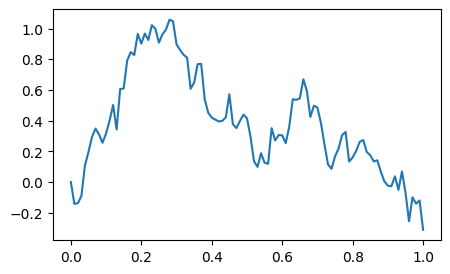
\includegraphics[width=7cm]{pic/bm-path.png}

Аналогичным образом можно симулировать сразу несколько траекторий.
Например, следующий фрагмент производит массив формы $(n+1, m)$, каждый столбец которого является одной траекторией геометрического броуновского движения с коэффициентом сноса $\mu$, волатильности $\sigma$ и начальным значением 1.
Мы воспользуется тем, что такой процесс является экспонентой броуновского движения со коэффициентом сноса $(mu-\frac12 sigma^2)$ и волатильности $\sigma$, и поэтому сначала будем симулировать траектории этого процесса, а затем применим функцию экспоненты. 
Следует обратить внимание на параметр \verb"axis=0", который используется для вычисления кумулятивной суммы приращений в каждом столбце по отдельности.

\begin{python}
### [numpy-basics.ipynb] ###
mu = 0
sigma = 1
m = 5

# Приращения всех траекторий броуновского движения со сносом
dX = rng.normal((mu - 0.5*sigma**2)*t/n, sigma*sqrt(t/n), (n, m))  
# Траектории броуновского движения со сносом
X = np.vstack((np.zeros(m), np.cumsum(dX, axis=0)))
# Траектории геометрического броуновского движения
S = np.exp(X)

# Если второй аргумент функции plot является 2-мерным массивом, то считается,
# что каждый столбец представляет собой отдельную функцию
plt.plot(T, S);
\end{python}

\noindent
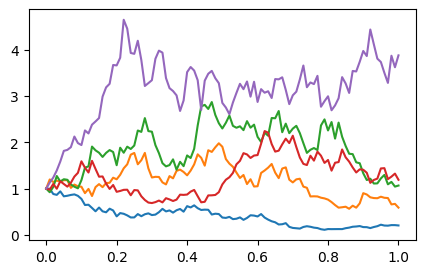
\includegraphics[width=7cm]{pic/gbm-paths.png}
